% Source: Code/ML_overlay/ir_rgb_registration/paper/ml_overlay_report_materials/ir_rgb_registration_report/figures/fig_cost_volume.tex
\documentclass[tikz,border=10pt]{standalone}
\usepackage{tikz}
\usetikzlibrary{arrows.meta,positioning,calc,patterns}

\definecolor{garnet}{RGB}{115,0,10}
\definecolor{rose}{RGB}{204,46,64}
\definecolor{atlantic}{RGB}{70,106,159}
\definecolor{congaree}{RGB}{31,65,77}
\definecolor{horseshoe}{RGB}{101,120,11}
\definecolor{black90}{RGB}{54,54,54}
\definecolor{black50}{RGB}{162,162,162}

\begin{document}
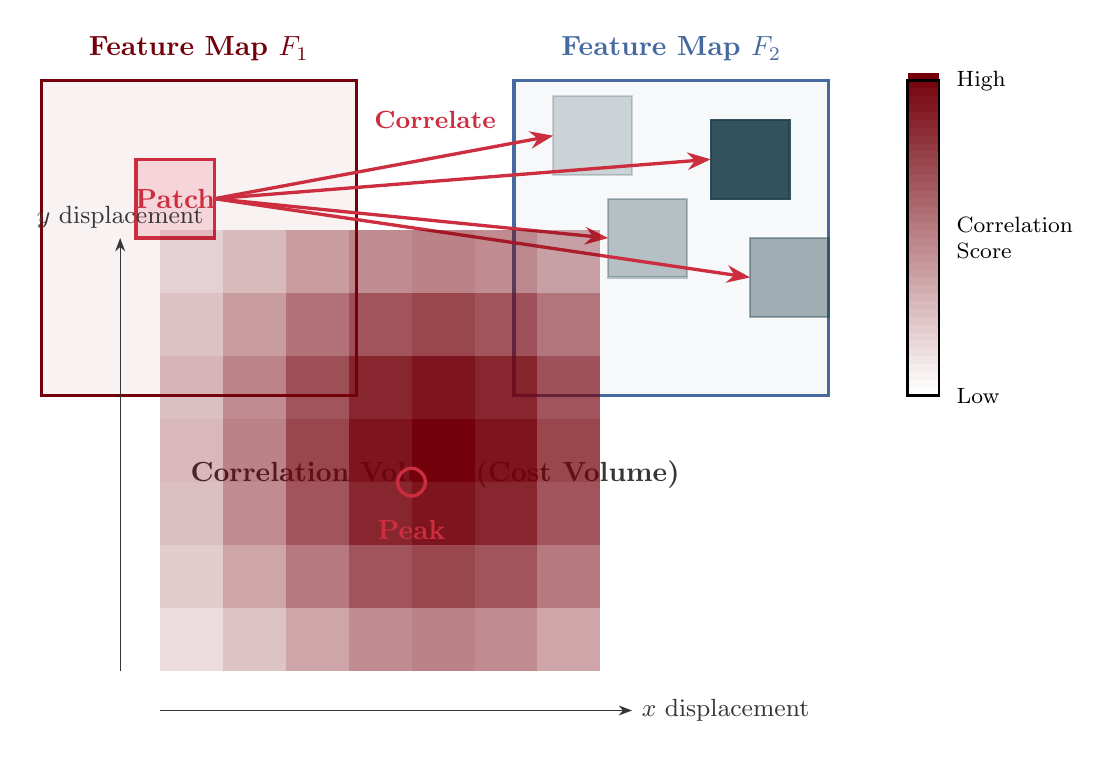
\begin{tikzpicture}[>=Stealth]

    % Feature map F1
    \draw[very thick, garnet, fill=garnet!5] (0,0) rectangle (4,4);
    \node[garnet, font=\bfseries] at (2,4.4) {Feature Map $F_1$};

    % Highlighted patch in F1
    \draw[very thick, rose, fill=rose!20] (1.2,2) rectangle (2.2,3);
    \node[rose, font=\bfseries] at (1.7,2.5) {Patch};

    % Feature map F2
    \draw[very thick, atlantic, fill=atlantic!5] (6,0) rectangle (10,4);
    \node[atlantic, font=\bfseries] at (8,4.4) {Feature Map $F_2$};

    % Search positions in F2
    \foreach \x/\y/\op in {6.5/2.8/0.2, 7.2/1.5/0.3, 8.5/2.5/0.9, 9/1/0.4} {
        \draw[thick, congaree, fill=congaree, opacity=\op] (\x,\y) rectangle (\x+1,\y+1);
    }

    % Correlation arrows
    \draw[->, very thick, rose] (2.2,2.5) -- (6.5,3.3);
    \draw[->, very thick, rose] (2.2,2.5) -- (7.2,2);
    \draw[->, very thick, rose] (2.2,2.5) -- (8.5,3);
    \draw[->, very thick, rose] (2.2,2.5) -- (9,1.5);

    \node[rose, font=\small\bfseries] at (5,3.5) {Correlate};

    % Correlation heatmap below
    \node[font=\bfseries, black90] at (5,-1) {Correlation Volume (Cost Volume)};

    \begin{scope}[shift={(1.5,-3.5)}]
        % Heatmap grid
        \foreach \x in {0,...,6} {
            \foreach \y in {0,...,6} {
                \pgfmathsetmacro{\val}{100*exp(-0.08*((\x-4)^2 + (\y-3)^2))}
                \pgfmathsetmacro{\opacity}{\val/100}
                \fill[garnet, opacity=\opacity] (\x*0.8,\y*0.8) rectangle (\x*0.8+0.8,\y*0.8+0.8);
            }
        }

        % Peak location
        \draw[rose, very thick] (3.2,2.4) circle (5pt);
        \node[rose, font=\bfseries] at (3.2,1.8) {Peak};

        % Axes
        \draw[->, black90] (0,-0.5) -- (6,-0.5) node[right, font=\small] {$x$ displacement};
        \draw[->, black90] (-0.5,0) -- (-0.5,5.5) node[above, font=\small] {$y$ displacement};

    \end{scope}

    % Color bar
    \begin{scope}[shift={(11,0)}]
        \foreach \i in {0,...,40} {
            \pgfmathsetmacro{\op}{\i/40}
            \fill[garnet, opacity=\op] (0,\i*0.1) rectangle (0.4,\i*0.1+0.1);
        }
        \draw[thick] (0,0) rectangle (0.4,4);
        \node[font=\footnotesize, right] at (0.5,4) {High};
        \node[font=\footnotesize, right] at (0.5,0) {Low};
        \node[font=\footnotesize, right, align=left] at (0.5,2) {Correlation\\Score};
    \end{scope}

\end{tikzpicture}
\end{document}
